\subsection*{Analyseklasser}
Inden analyseklasserne udarbejdes, foretages en analyse ud fra systembeskrivelsen, use case og funktionaliteter til at identificere substantiver og verber. Dette gøres for at sikre, at alle funktionaliteter indgår i klassediagrammet. Substantiver og verber fremgår af \autoref{tab:subverb}.

\begin{table}[H]
\centering
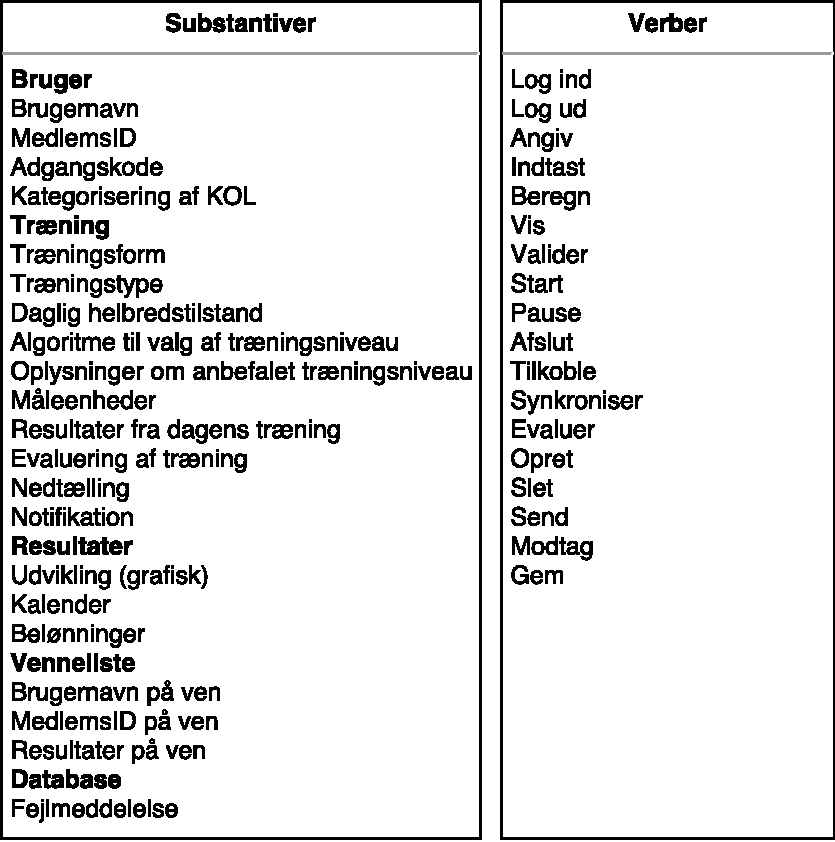
\includegraphics[width=0.7\textwidth]{figures/aktivitetsdiagram/substantiveverber}
\caption{Substantiver og verber identificeret ved analyse af systembeskrivelse, use case samt funktionaliteter.}
\label{tab:subverb}
\end{table}

\noindent
De fremhævede substantiver, brugeroplysninger, træning, resultater, venneliste og database, identificeres som klasser. Under hver klasse fremgår deres tilhørende attributter, der beskriver den overordnede klasse. Verberne betegner de metoder, der kan tilgås i de forskellige klasser. 


\subsubsection{Analyseklasse stereotyper}
Analyseklasser kan inddeles i tre stereotyper, herunder entity, boundary og control, hvilket er et værktøj til at identificere klasser i analyse og tidlig designfase \cite{RSC2002}.

\begin{itemize}
\item Entity anvendes til at lagre og opdatere informationer om objekter. Dens attributværdier gives ofte af en aktør.\cite{RSC2002}
\item Boundary anvendes til interaktion mellem bruger og system og sikre at ændringer i boundary ikke påvirker resten af systemet \cite{RSC2002}.
\item Control anvendes til at kontrollere handlinger \cite{RSC2002}. 
\end{itemize}

\noindent
Efter analyseklasserne er identificeres i  \autoref{tab:subverb} inddeles disse i analyseklasser og opdeles i stereotyper. Dette kan ses af \autoref{fig:analyseklasse}. 

\begin{figure}[H]
\centering
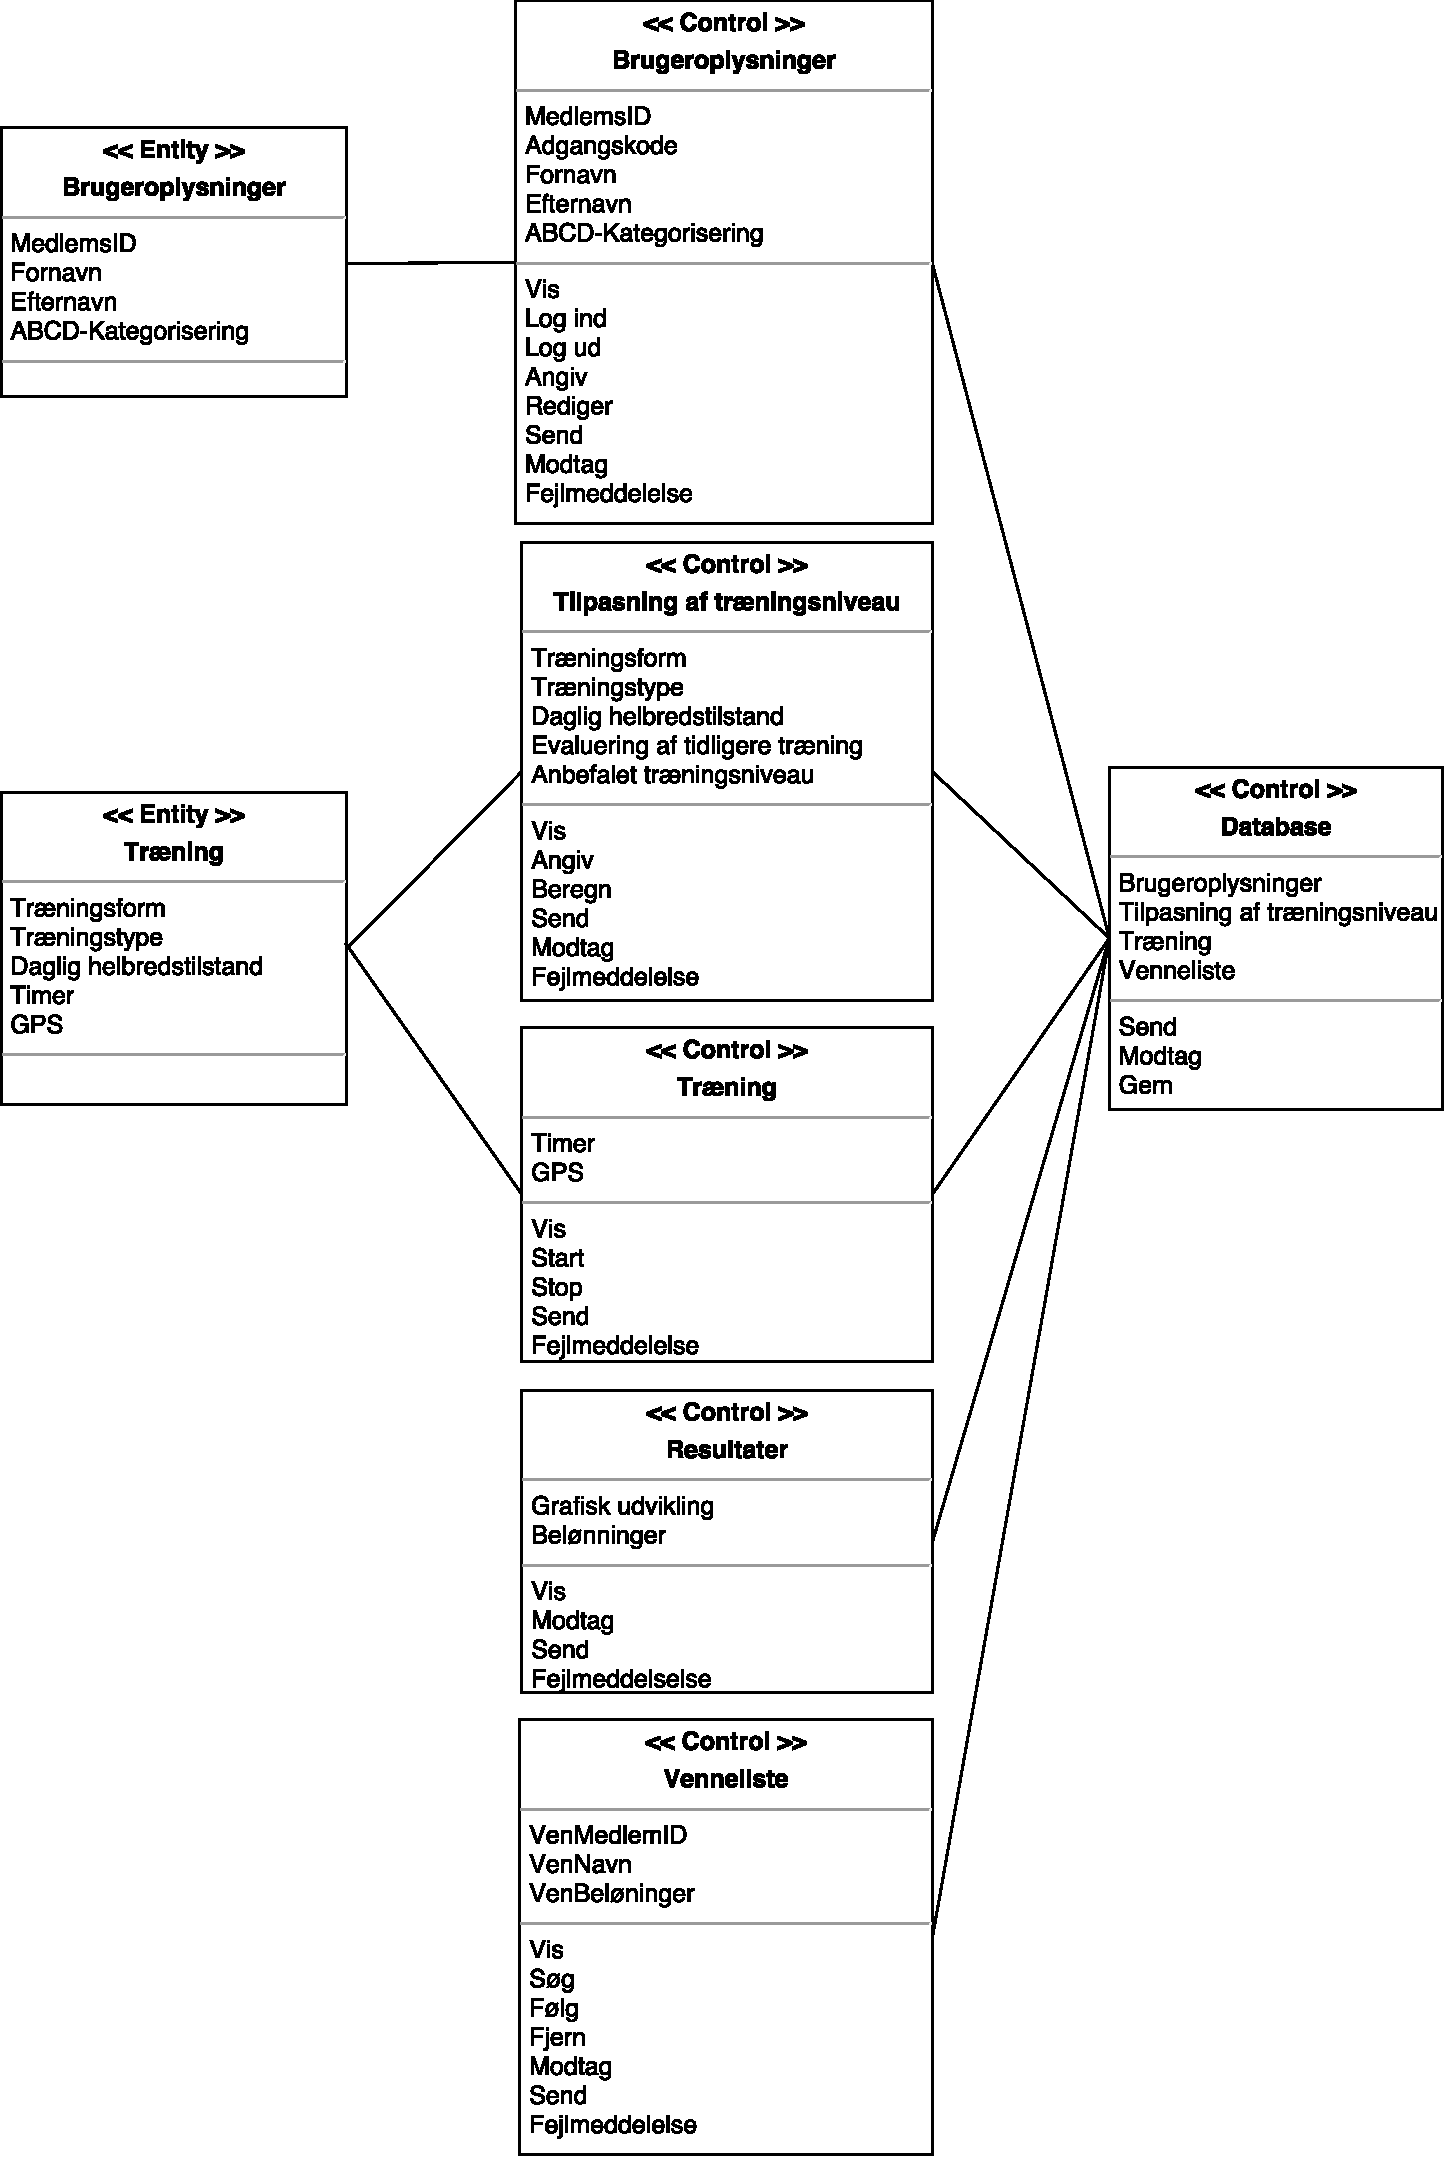
\includegraphics[width=0.7\textwidth]{figures/aktivitetsdiagram/analyseklasser}
\caption{Analyseklasser udarbejdet ud fra de identificerede substantiver og verber.}
\label{fig:analyseklasse}
\end{figure}

\noindent
Af \autoref{fig:analyseklasse} fremgår relationen mellem klasserne og deres tilhørende attributter samt metoder.  \textit{Database} er defineret som entityklasser, da de skal lagre og opdatere informationer. \textit{Resultater} er defineret som boundaryklasse, da den skal vise resultater på grænseflade.  \textit{Brugeroplysninger}, \textit{Tilpasning af træningsniveau}, \textit{Træning} og \textit{Venneliste} defineres som controlklasser, idet disse anvendes til at kontrollere handlinger. 

